\documentclass{standalone}

\usepackage{pgfplots}
\pgfplotsset{compat=1.10}   % in my packages used compat=1.15
\usepgfplotslibrary{fillbetween}
\usepackage{pgf}
\usepackage{tikz}
\usetikzlibrary{patterns,arrows,calc,decorations.pathmorphing,backgrounds, positioning,fit,petri,decorations.fractals}
\usetikzlibrary{matrix}

\usepackage[table,dvipsnames]{tudscrcolor}

\usepackage[default]{opensans}

\begin{document}
	\color{cddarkblue}
	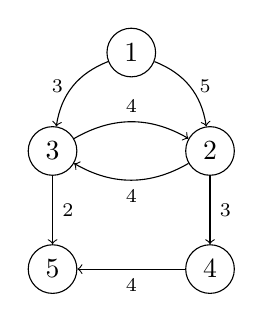
\begin{tikzpicture}[auto]
	% Knoten
		\node (1) at (0,2)  [circle,draw] {1};
		\node (3) at (-1,.75) [circle,draw] {3};
		\node (5) at (-1,-.75) [circle,draw] {5};
		\node (2) at (1,.75) [circle,draw] {2};
		\node (4) at (1,-.75) [circle,draw] {4};
	% Kanten
%		\path (1) -> node[weight] {$3$} (3)
		\draw[->, bend left]  (1) edge node[right]{\scriptsize 5} (2);
		\draw[->, bend right] (1) edge node[left]{\scriptsize 3} (3);
		\draw[->, bend left] (3) edge node[above]{\scriptsize 4} (2);
		\draw[->, bend left] (2) edge node[below]{\scriptsize 4} (3);
		\draw[->] (2) edge node{\scriptsize 3} (4);
		\draw[->] (4) edge node{\scriptsize 4} (5);
		\draw[->] (3) edge node{\scriptsize 2} (5);
	\end{tikzpicture}
\end{document}